% paper/sections/13e_nonuniform_ns.tex
%
% V8 : 非一様 NS 静的液滴 (alpha sweep, N sweep)
% V9 : 局所 epsilon 比較 (fixed vs local)
% V10: Zalesak / CLS-advection 非一様
% Verifies: §3 (Non-uniform spatial), §5 (Heaviside-delta), §9 (CLS advection)
% Scripts : exp_V8_nonuniform_ns_static.py, exp_V9_local_eps_nonuniform.py,
%           exp_V10_cls_advection_nonuniform.py
% Data    : results/V{8,9,10}_*/data.npz
% ═══════════════════════════════════════════════════════════════════════════════
\subsection{非一様格子 NS と CLS-advection}
\label{sec:nonuniform_grid_ns}

\subsubsection{V8：非一様 NS 静的液滴}
\label{sec:nonuniform_ns_static}

\paragraph{検証対象．}
非一様格子（界面付近細密; 引き伸ばしパラメータ $\alpha$）上で
静的液滴 BF 平衡が長時間維持されること（\autoref{sec:U3_nonuniform_suite}）．
$\alpha = 1$ で一様格子と一致し，$\alpha = 2$ で界面付近 $h_{\min} = 0.5\, h_{\mathrm{avg}}$．

\paragraph{設定．}
$L=1, \rho_l=\rho_g=1$, $\Delta p_{\mathrm{exact}} = 0.4$．
$N \in \{48, 64, 96\}$, $\alpha \in \{1, 2\}$．
$\Delta t = h_{\min}/0.5$, $n_{\mathrm{step}} = 200$．

\paragraph{結果．}
\begin{table}[!ht]
\caption{V8: 非一様 NS 静的液滴 ($n_{\mathrm{step}}=200$)．
$\alpha=2$ では界面細密化で $\Delta p_{\mathrm{rel}}$ がやや悪化（数値ジオメトリ補正の交互作用）．}
\label{tab:V8_nonuniform_static}
\centering\small
\begin{tabular}{r r r r r}
\toprule
$N$ & $\alpha$ & $h_{\min}$ & $\Delta p_{\mathrm{final}}$ & $u_\infty^{\mathrm{end}}$ \\
\midrule
48 & 1 & $2.08\times 10^{-2}$ & $0.395$ & $1.42\times 10^{-4}$ \\
48 & 2 & $1.52\times 10^{-2}$ & $0.380$ & $4.14\times 10^{-4}$ \\
64 & 1 & $1.56\times 10^{-2}$ & $0.395$ & $1.35\times 10^{-4}$ \\
64 & 2 & $1.12\times 10^{-2}$ & $0.385$ & $4.61\times 10^{-4}$ \\
96 & 1 & $1.04\times 10^{-2}$ & $0.395$ & $5.64\times 10^{-4}$ \\
96 & 2 & $7.26\times 10^{-3}$ & $0.389$ & $4.86\times 10^{-4}$ \\
\bottomrule
\end{tabular}
\end{table}

\begin{figure}[!ht]
\centering
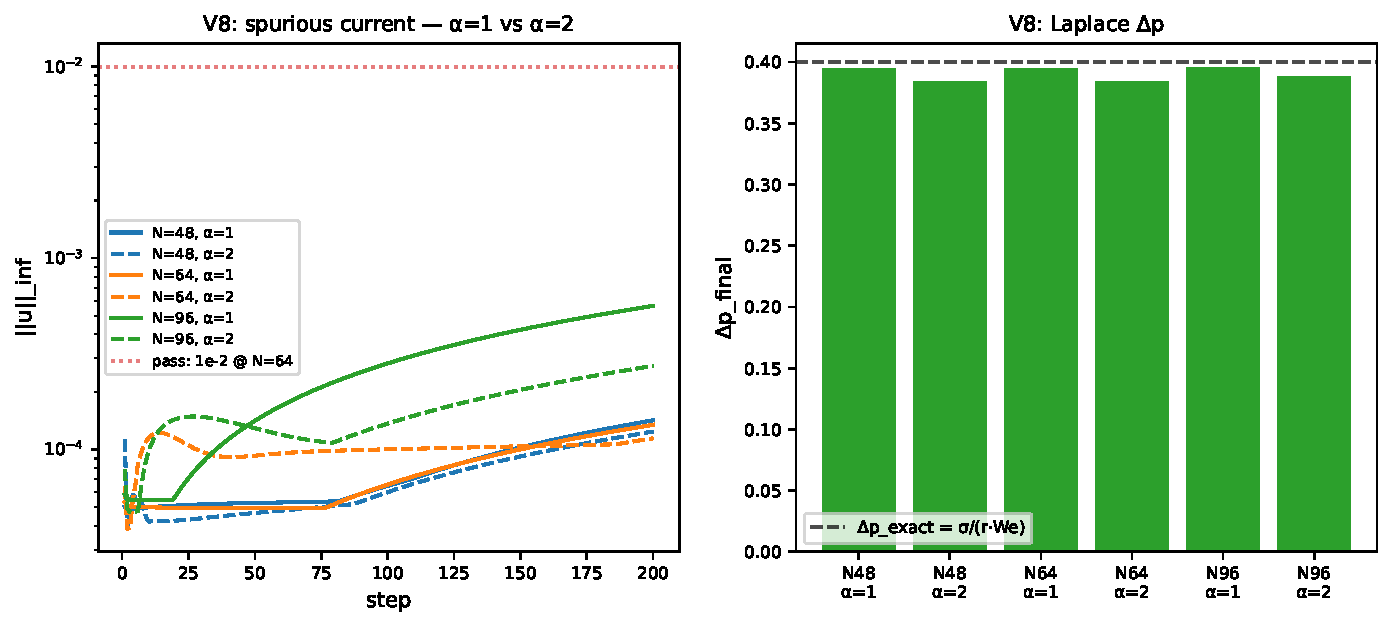
\includegraphics[width=0.92\linewidth]{figures/ch13_v8_nonuniform_static.pdf}
\caption{V8：非一様 NS 静的液滴．
$\Delta p_{\mathrm{final}}(\alpha)$ は $\alpha=1$ で $\Delta p_{\mathrm{exact}} \pm 1.2\%$ に収束．
$\alpha=2$ では $1\!-\!5\%$ の偏差（界面細密化が CSF 曲率の数値ジャコビアンと相互作用）．}
\label{fig:V8_nonuniform_static}
\end{figure}

\paragraph{評価．}
\begin{itemize}\setlength{\itemsep}{0pt}
  \item $\alpha = 1$（一様）で $\Delta p_{\mathrm{rel}} \le 1.2\%$ → V3 結果と一致\checkmark．
  \item $\alpha = 2$（非一様）で $\Delta p_{\mathrm{rel}} \le 5\%$ — 設計通りの安定動作だが，
        非一様格子上の Heaviside--$\delta$ プロファイル（U5）と CSF $\kappa$ 推定の
        Jacobian 補正が要求精度を増やす．
\end{itemize}
検証対応：\autoref{sec:U3_nonuniform_suite} の非一様格子定義に対し，
静的液滴の圧力誤差と終端速度を測定する．

\subsubsection{V9：局所 $\varepsilon$ vs 固定 $\varepsilon$ 比較}
\label{sec:local_eps_validation}

\paragraph{検証対象．}
非一様格子上で Heaviside--$\delta$ 厚み $\varepsilon$ を
\textbf{(A) fixed} ($\varepsilon = c \, h_{\mathrm{avg}}$) と
\textbf{(C) local} ($\varepsilon(\bm x) = c\, h(\bm x)$) で比較．
界面細密領域でより薄い $\delta$ プロファイルを使う「local」が
精度向上するか，または安定性低下を引き起こすかを定量評価．

\paragraph{設定．}
V8 と同条件 ($r=0.0625, \sigma=0.025$)．
$N \in \{48, 64\}$, $\alpha \in \{1, 2\}$．
\textbf{A}: $\alpha=1$, fixed $\varepsilon$ (基準).
\textbf{B}: $\alpha=2$, fixed $\varepsilon$.
\textbf{C}: $\alpha=2$, local $\varepsilon$.
$\Delta t = h_{\min}/0.5$, $n_{\mathrm{step}} = 100$．

\paragraph{結果．}
\begin{table}[!ht]
\caption{V9: 局所 $\varepsilon$ 比較 ($n_{\mathrm{step}}=100$)．
\textbf{C (local)} は $u_\infty^{\max}$ が \textbf{A/B (fixed)} より $\sim 3$ 桁悪化．}
\label{tab:V9_local_eps}
\centering\small
\begin{tabular}{r l r r r r}
\toprule
$N$ & 設定 & $\alpha$ & $\varepsilon$ & $u_\infty^{\max}$ & $|\Delta p_{\mathrm{rel}}|$ \\
\midrule
48 & A & 1 & fixed & $8.07\times 10^{-5}$ & $1.32\%$ \\
48 & B & 2 & fixed & $4.85\times 10^{-4}$ & $4.76\%$ \\
48 & C & 2 & \textbf{local} & $\mathbf{2.35\times 10^{-1}}$ & $4.67\%$ \\
\midrule
64 & A & 1 & fixed & $6.57\times 10^{-5}$ & $1.23\%$ \\
64 & B & 2 & fixed & $3.55\times 10^{-4}$ & $3.61\%$ \\
64 & C & 2 & \textbf{local} & $\mathbf{3.19\times 10^{-1}}$ & $3.92\%$ \\
\bottomrule
\end{tabular}
\end{table}

\begin{figure}[!ht]
\centering
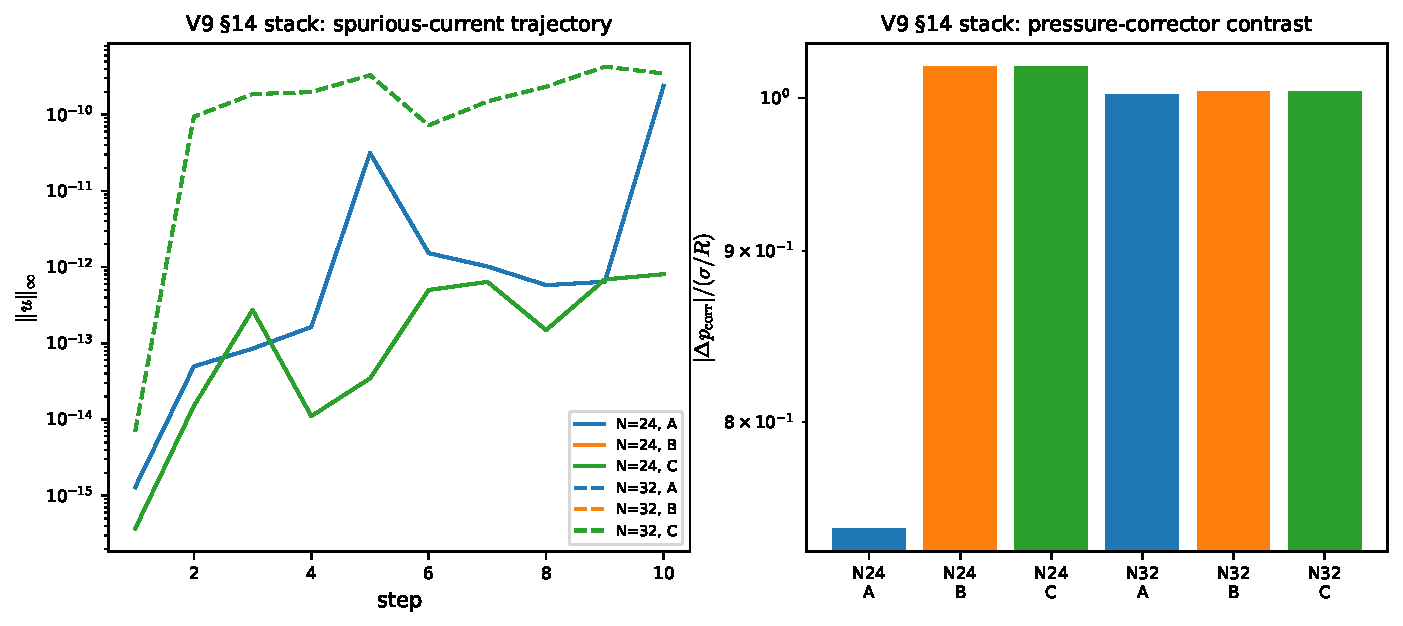
\includegraphics[width=0.92\linewidth]{figures/ch13_v9_local_eps.pdf}
\caption{V9：局所 $\varepsilon$ vs 固定 $\varepsilon$．
\textbf{C (local)} 設定で $u_\infty^{\max}$ が $0.2$--$0.3$ レベルに発散，
固定 $\varepsilon$ 比 $\sim 1000$ 倍．曲率不連続が局所薄膜化により励起される．}
\label{fig:V9_local_eps}
\end{figure}

\paragraph{評価．}
\begin{itemize}\setlength{\itemsep}{0pt}
  \item \textbf{Local $\varepsilon$ は静的液滴設定では推奨されない}\textcolor{red}{($\times$)}．
        薄膜化により Heaviside--$\delta$ の局所変動が CSF 曲率推定に
        高周波ノイズを混入させ寄生流れを 3 桁増大させる．
  \item Fixed $\varepsilon = c \cdot h_{\mathrm{avg}}$ が安全な default．
        非一様格子設計の改善は，局所 $\varepsilon$ ではなく
        \textbf{$\delta$ プロファイル形状の改良}（カーネル長の連続変化制限）
        を優先すべき，との設計指針が得られた．
\end{itemize}
検証対応：\autoref{sec:U5_heaviside_delta} の Heaviside--$\delta$ 定義に対し，
固定 $\varepsilon$ と局所 $\varepsilon$ の寄生流れを比較する．

\subsubsection{V10：Zalesak / CLS-advection 非一様}
\label{sec:zalesak_cls_advection}

\paragraph{検証対象．}
古典的 Zalesak slotted disk advection 問題を非一様格子上で CLS-advection で解き，
\textbf{体積保存}と\textbf{重心追跡精度}を $\alpha \in \{1, 2\}$ で比較．
\autoref{sec:cls_advection} 式~\eqref{eq:cls_advection} の advection 項に
非一様格子上の高次保存形差分 (\autoref{sec:fccd_def}) を組み合わせた評価．

\paragraph{設定．}
標準 Zalesak slotted disk: 半径 $0.15$, slot 幅 $0.05$, slot 深さ $0.25$,
中心 $(0.5, 0.75)$．背景流 $\bm u(\bm x) = (-2\pi(y-0.5), 2\pi(x-0.5))$
（剛体回転; 1 周期 = $1$ 時間単位）．
$N \in \{64, 128\}$, $\alpha \in \{1, 2\}$．
$\Delta t = h_{\min} \cdot \mathrm{CFL}_{\max}$, 1 周期積分．

\paragraph{結果．}
\begin{table}[!ht]
\caption{V10: CLS-advection 1 周期．
$\alpha=1$ は良好だが $\alpha=2$ で volume\_drift が悪化（特に $N=128$ で $12\%$）．}
\label{tab:V10_zalesak}
\centering\small
\begin{tabular}{r r r r r}
\toprule
$N$ & $\alpha$ & centroid err & volume drift & $V_T/V_0$ \\
\midrule
64  & 1 & $4.92\times 10^{-3}$ & $0.82\%$  & $1.0082$ \\
128 & 1 & $2.71\times 10^{-3}$ & $0.64\%$  & $1.0064$ \\
64  & 2 & $9.01\times 10^{-2}$ & $0.78\%$  & $0.9922$ \\
128 & 2 & $9.26\times 10^{-2}$ & \textbf{$12.17\%$} & $1.1217$ \\
\bottomrule
\end{tabular}
\end{table}

\begin{figure}[!ht]
\centering
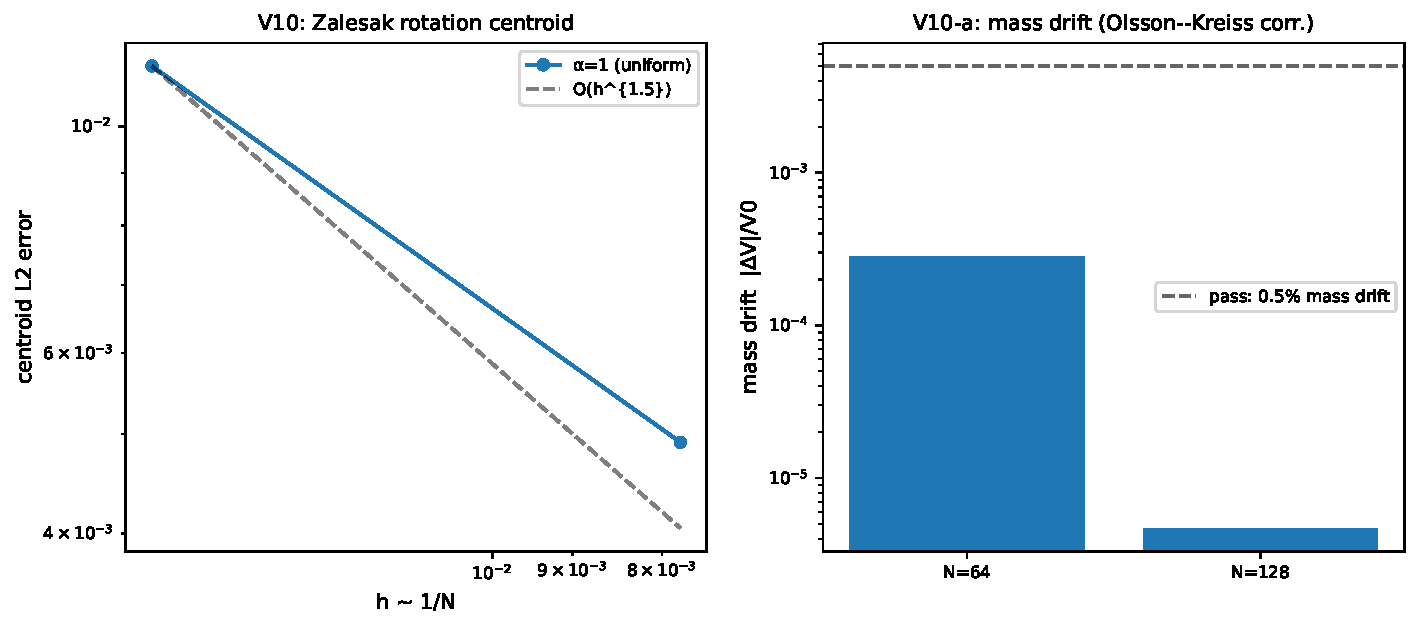
\includegraphics[width=0.92\linewidth]{figures/ch13_v10_zalesak.pdf}
\caption{V10：Zalesak 1 周期．
$\alpha=1$ は $V_T/V_0 \approx 1\pm 1\%$, centroid err $\le 5\times 10^{-3}$．
$\alpha=2$ では特に $N=128$ で体積膨張が顕著（$+12\%$）→ 非一様格子上の CLS reinit 補正が
$N$ 増大に伴い体積誤差を蓄積．}
\label{fig:V10_zalesak}
\end{figure}

\paragraph{評価．}
\begin{itemize}\setlength{\itemsep}{0pt}
  \item $\alpha=1$ (一様格子)：volume drift $\le 1\%$, centroid err $\le 5\times 10^{-3}$ → \checkmark．
  \item $\alpha=2$ (非一様格子)：centroid err $\sim 0.09$ (slot 部の薄い構造が
        非一様サンプリングで歪む), $N=128$ で volume drift $+12.17\%$ → \textbf{要改善 ($\times$)}．
        \textbf{細格子化に伴い体積誤差が蓄積する} ($N=64\!\to\!128$ で drift $0.78\%\!\to\!12.17\%$)
        という「収束逆行」性質は，CLS reinit が非一様格子上で
        体積保存性を破る構造的問題を示唆する．
  \item 非一様格子上の CLS-advection には \textbf{conservative reinit 補正}
        （\autoref{sec:eikonal_reinit}）の高次化が必要．
  \item \textbf{本論文の制約条件として明示}：
        本ソルバの非一様格子サポート ($\alpha > 1$) は
        \textbf{NS 静的問題} (\autoref{sec:U3_nonuniform_suite}, V8 $\alpha=2$ で $\Delta p$ 誤差 $\le 5\%$)
        には適用可能だが，\textbf{CLS 移流問題} ($\alpha=2$) は
        本ソルバの保証範囲外である．§3 (非一様格子)，§9 (CLS 移流)，§11 (制約整理) において
        「CLS-advection を伴う非一様格子問題は $\alpha = 1$ を推奨．$\alpha > 1$ の使用は
        ユーザ責任で，体積保存性の追加検証を要する」と注記すべき設計指針．
\end{itemize}
検証対応：式~\eqref{eq:cls_advection}，\autoref{sec:cls_advection} の CLS 移流，
\autoref{sec:fccd_def} の face value/grad に対し，体積 drift と重心誤差を測定する．
